% !TeX root = ../main.tex
\chapter{Introduction}\label{chapter:introduction}

\section{Motivation}\label{section:motivation}

\gls{VR} is an emerging technology, which provides new ways to present and interact with digital information. \citeauthor{Sherman.2003} define \gls{VR} by the four key elements virtual world, immersion, sensory feedback, and interactivity. They define the virtual world as an imaginary space which may be manifested through a medium. It is also a description of objects in a space together with rules and relationships. According to the authors, immersion means the feeling of presence in a virtual world. An essential ingredient to \gls{VR} is the sensory feedback, which describes the feedback the \gls{VR} system conveys to the user depending on the user's state in the virtual world. \gls{VR} should respond to the user's actions to make it interactive, in order for \gls{VR} to seem authentic.

These four elements form the definition as a medium composed of interactive computer simulations that may sense the user's behavior and replace or augment the sensory feedback, with the goal of immersing the user in a virtual world~\cite[6-12]{Sherman.2003}.

% TODO: übergang in order to immersiv
A \gls{HMD} as the display device, connected to a \gls{PC} which processes the data, is required for modern consumer \gls{VR} systems. Often an external tracking system is presumed, too. An application, rendering \gls{3D} content, similar to a computer game, is required to present a so-called \gls{VE} to the user.

% while the ve can display... great experience: non academic
Exploring \glspl{VE} is a great experience. However, \gls{VR} really shines when interactivity comes into play. Since consumer \glspl{HMD} are now available, the development of tracked hand controllers (also known as \gls{VR}/\gls{3D}/hand/motion controllers) gets more important.
Best practices are not yet defined, which leaves much room for new methods and research. Figure~\ref{fig:vr-controllers} illustrates the variety of different consumer \gls{VR} controllers available.

\begin{figure}[H]%
	\centering%
	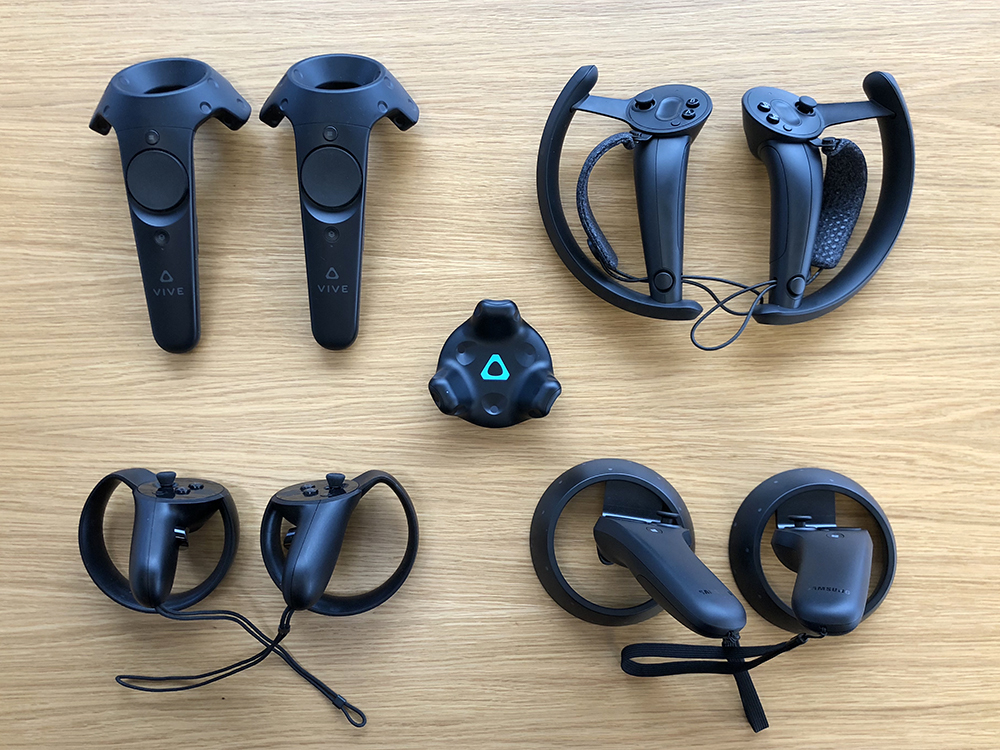
\includegraphics[width=10cm]{figures/introduction/vr_controllers.jpg}%
	\caption[Collection of VR controllers]{A collection of different \gls{VR} controllers. From left to right, top to bottom: HTC VIVE Controllers, Valve Index Controllers (\enquote{Knuckles}), VIVE Tracker, Oculus Touch Controllers, Samsung Odyssey Controllers~\cite{Yang.2018}.}\label{fig:vr-controllers}
\end{figure}

Mapping the movement of our real hands to the virtual world is a common strategy in current \gls{VR} hardware. Not only does it enhance the virtual presence by showing the user a representation of his body, but it also gives the user a natural way of controlling and interacting with the virtual world.

The Leap Motion\footnote{The Leap Motion controller is a hand tracking device, which is often used to display a hand avatar. Website: \href{https://www.leapmotion.com/}{www.leapmotion.com}} sensor uses multiple infrared cameras to track hand poses, which is only possible in front of the sensor. Newer generations of \gls{VR} controllers try to achieve a similar effect with different methods: The Oculus Touch\footnote{The Oculus Touch controllers are hand tracking devices included with the Oculus Rift \gls{HMD}. Website: \href{https://www.oculus.com/rift/}{www.oculus.com/rift}} controllers track the distance of the fingers from the controller and the Valve Index\footnote{The Valve Index is a \gls{HMD} which includes its own set of controllers, called \enquote{Knuckles}. Website: \href{https://store.steampowered.com/valveindex}{store.steampowered.com/valveindex}} controllers even have pressure sensors built-in.

However, for many interactions, hand inspired controllers are not ideal. This applies especially to productive \gls{VR} applications, which require interactions like inputting text for labeling or manipulating \gls{3D} shapes. Most \gls{VR} controllers also require complex external tracking systems.

The Google Cardboard\footnote{The Google Cardboard is a \gls{HMD} made out of cardboard, which uses a smartphone as a display and for tracking. Website: \href{https://vr.google.com/cardboard/}{vr.google.com/cardboard}} uses a smartphone as a display and as a tracking device. This demonstrates the versatility of smartphones. Most people already have one, since they are portable general-purpose devices and are not very expensive anymore. Thanks to \gls{WLAN} and Bluetooth\footnote{Bluetooth is a wireless standard for exchanging data over short ranges between mobile devices.} it is easy to connect the smartphone to other devices.

Smartphones have input devices like buttons, a touch screen, an \gls{IMU}\footnote{An IMU is an electronic component which is part of most smartphones and allows to measure a specific force, angular rate, and magnetic field.}. But also, output devices like the display, vibration motors and speakers are present. This makes them similar to \gls{VR} controllers.

One significant difference between smartphones and common \gls{VR} controllers is that smartphones are not capable of accurate positional tracking. The position can be estimated using the data of an \gls{IMU}, but since the error accumulates over time~\cite[44]{Steed.2013}, this method cannot be used. Additional tracking methods, like using the \gls{WLAN} signal strength, can be used to correct the drift~\cite{Zhang.2015}. However, those methods are still not good enough, because \gls{VR} requires very accurate tracking with short distances.
Besides the missing positional tracking, the other advantages lead to the assumption that the smartphone can be used as an alternative \gls{VR} controller.


\section{Problem Statement}\label{section:problem-statement}
This thesis aims to explore the possibilities of using the smartphone as an interaction device in \gls{VR} experiences. The fundamental question is, whether smartphones are useable as \gls{VR} input devices.

% were implemented instead of was im
To answer that question, some promising typical \gls{VR} interaction methods have to be implemented using a smartphone. The goal of those experiments is not to create a better system, but rather show that the smartphone can be used as well as common \gls{VR} controllers for specific interactions.

%also change time here
To benchmark the performance, a user study should be performed where participants complete tasks using the prosed input systems.
The performance of the users in those tasks should be evaluated and, if possible, compared with similar methods from other research.

Additionally, a \gls{SUS} user study should be performed to get an assessment of the user's feel for the interface.
\gls{UBII} architecture should be used to implement an abstracted and reusable system.


\section{Outline}\label{section:outline}
% say chapter number; 
In the next chapter, different input methods using a smartphone or similar device from previous research is highlighted. The \gls{UBII} components and architecture, as well as the web-based technology stack used in this project, is then introduced and broken down. Afterward, different methods of using the smartphone as an alternative input device for typical \gls{VR} interactions are going to be introduced. In the fifth chapter, tasks to benchmark the user's performance are then described. The user study and its results are presented afterward. Following the evaluation of the user study results, a final conclusion is drawn.